\documentclass{article}
\usepackage{blindtext}
\usepackage[utf8]{inputenc}
\usepackage{graphicx}
\usepackage{hyperref}
\usepackage[dvipsnames]{xcolor}
\usepackage{fancyvrb}
\graphicspath{ {/home/abhinav/Desktop/} }
\usepackage{mathtools}
\DeclarePairedDelimiter{\ceil}{\lceil}{\rceil}
\DeclarePairedDelimiter{\floor}{\lfloor}{\rfloor}

\hypersetup{
     breaklinks=true,
     bookmarksopen=true,
     bookmarksnumbered=true,
     linkcolor=blue,
     urlcolor=blue,
     citecolor=blue,
     colorlinks=true}
\title{\textbf{General Linear Congruence Generator}}
\author{Abhinav Gupta}
\date{\today}

\begin{document}
 \tableofcontents
\maketitle

\section{Short Summary}
\ \ \ \ \ "\(y\ mod\ m\) can be implemented as \(y-(y/m) · m\)".

It can be shown that to avoid overflow a straight forward
implementation of a linear congruential generator in integer
variables must be restricted to small modulus.

\[ax_i mod m = a(x_i mod q)-\floor{x_i/q}r+(\floor{x_i/q}-\floor{ax_i/m})m\]

--\(>\)\ In this case the last term \((\floor{x_i/q}-\floor{ax_i/m})m\) has value either 0 or m.\
Therefore the last term is m precisely when \(a(x_i mod q)-\floor{x_i/q}r < 0\).

\section{Question-1}

\item \textbf{Uniform Look-alike distribution}
\item \textbf{The picture shows that the generated numbers are correct, since and n increasing we are getting
the proper shape of uniform distribution}
\begin{itemize}
\item a=16807\ \ \(m=2^{31}-1\)\
count=\ 1000


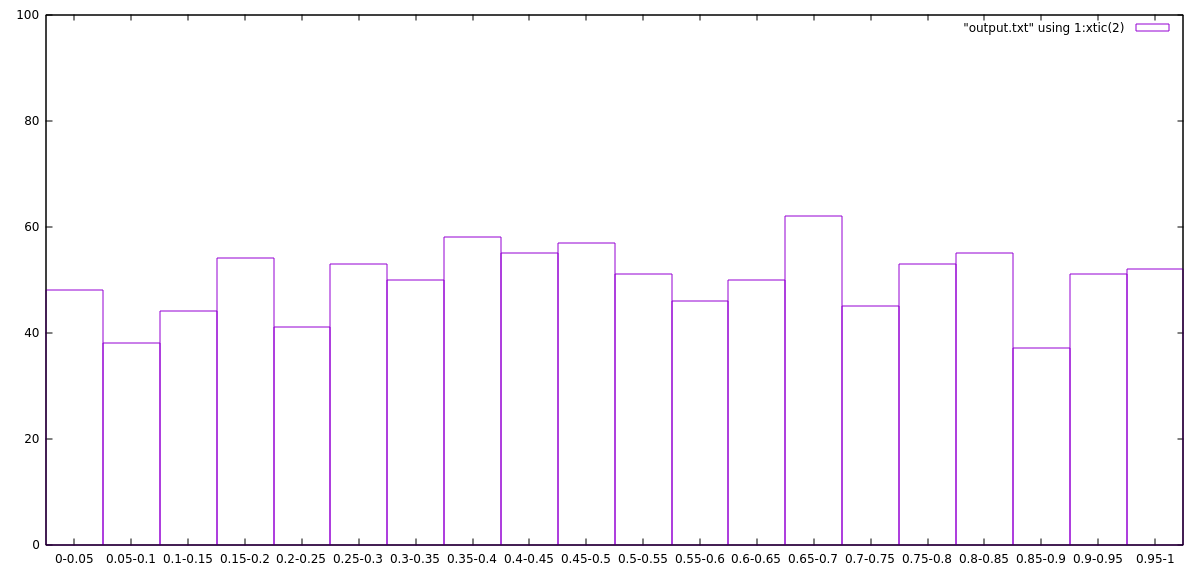
\includegraphics[scale=0.45]{a-1}
count=\ 10000


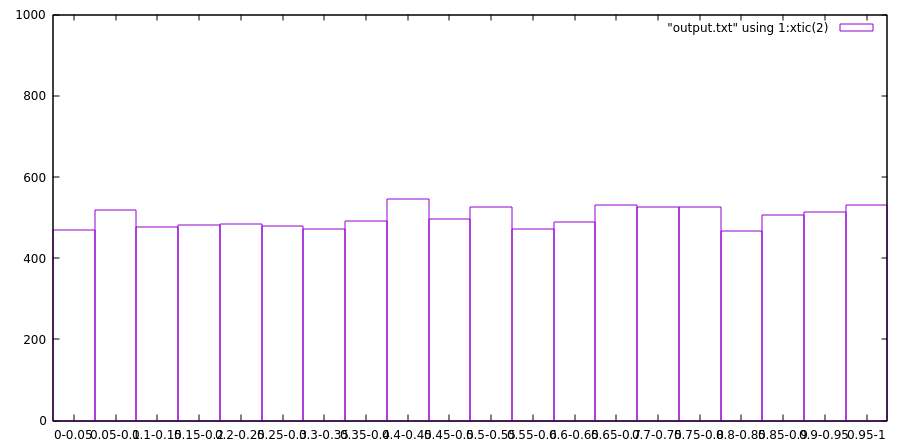
\includegraphics[scale=0.6]{a-2}
count=\ 100000


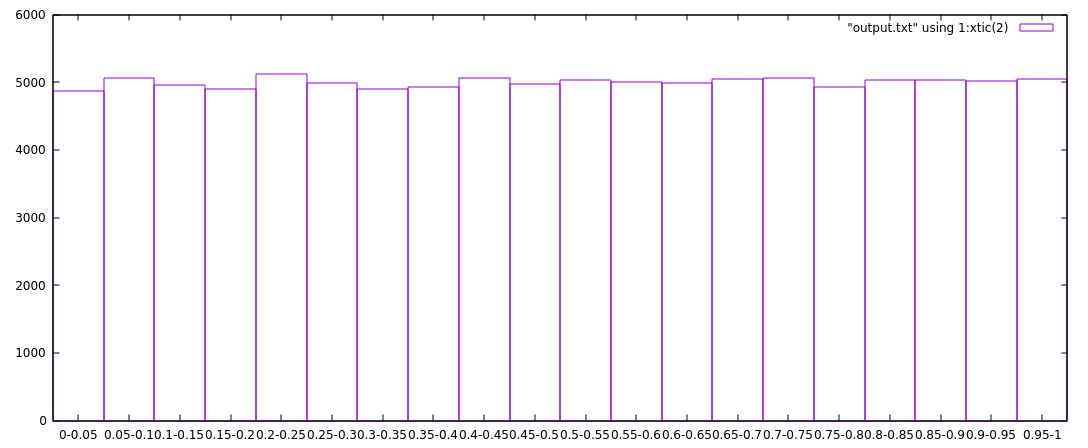
\includegraphics[scale=0.5]{a-3}
\item a=40692\ \ \(m=2147483399\)\
count=\ 1000


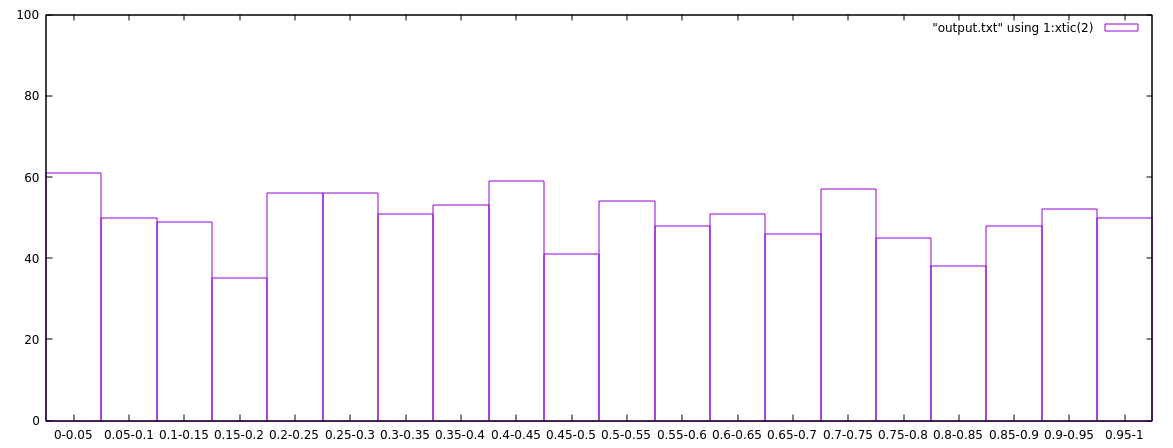
\includegraphics[scale=0.5]{b-1}
count=\ 10000


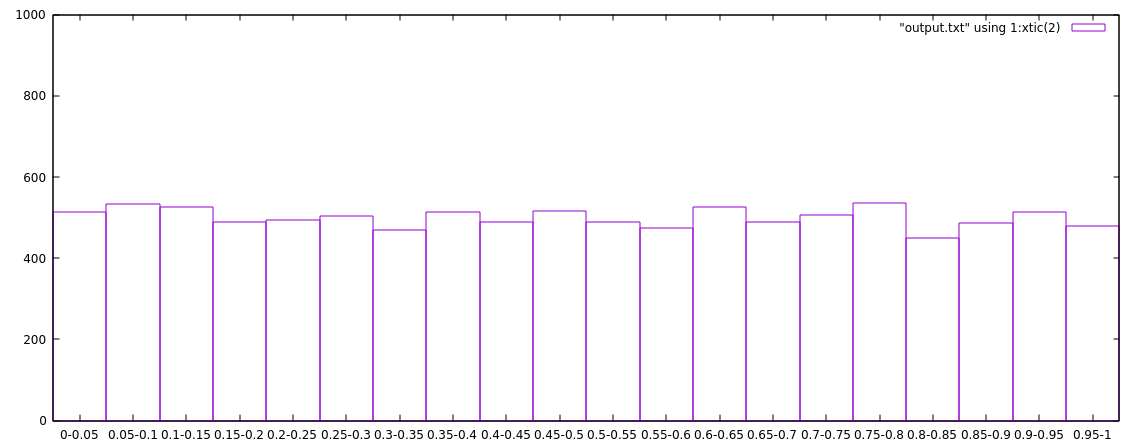
\includegraphics[scale=0.5]{b-2}
count=\ 100000


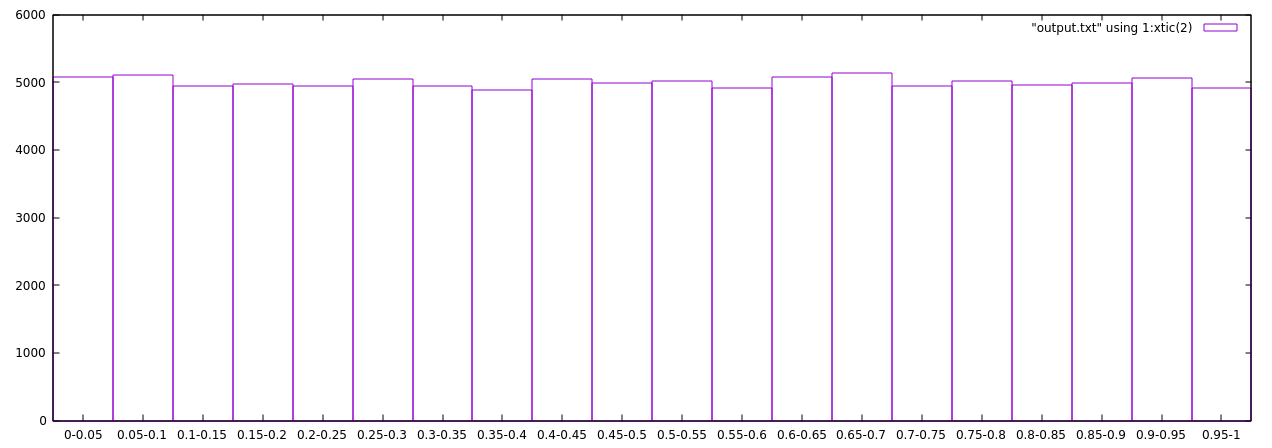
\includegraphics[scale=0.4]{b-3}
\item a=40014\ \ \(m=2147483563\)\
count=\ 1000


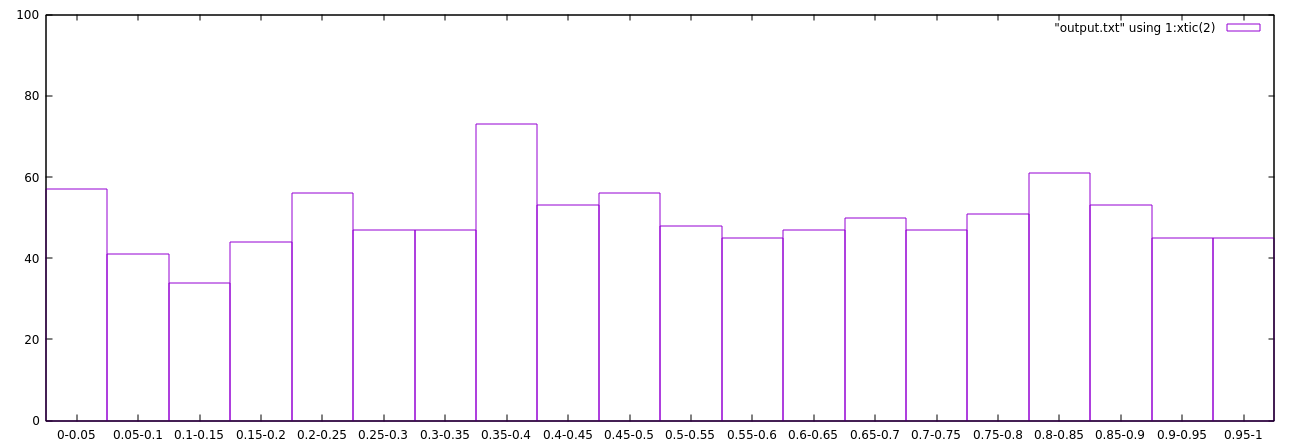
\includegraphics[scale=0.4]{c-1}
count=\ 10000


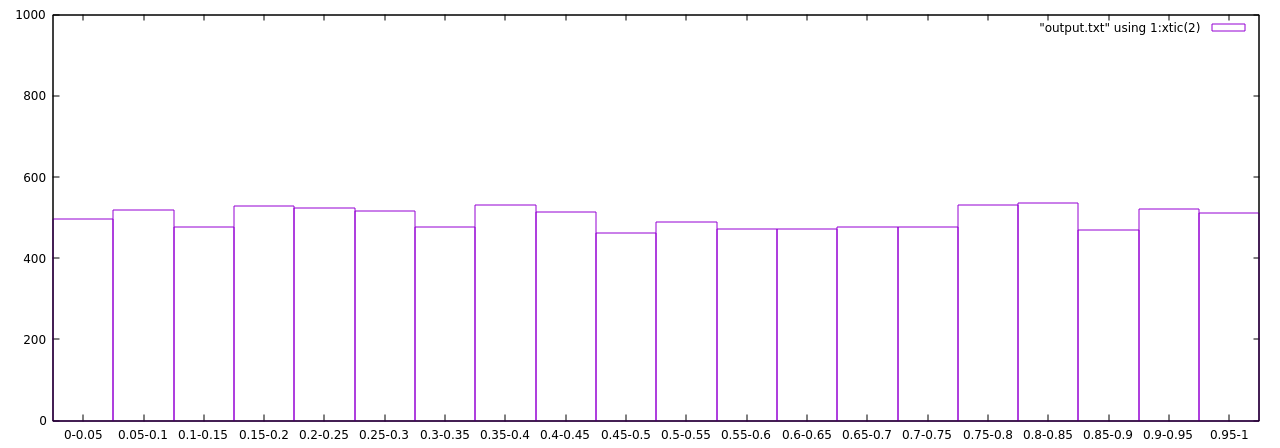
\includegraphics[scale=0.4]{c-2}
count=\ 100000


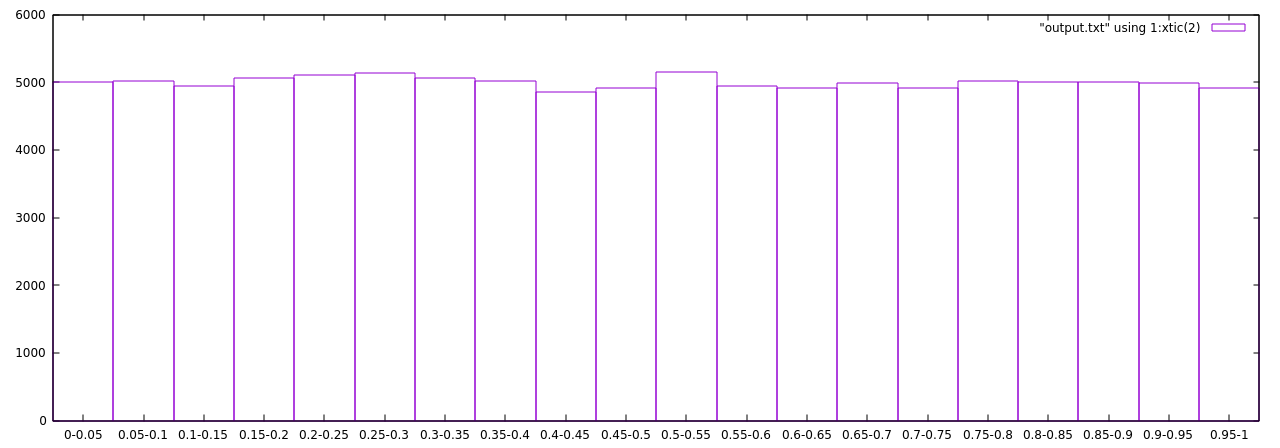
\includegraphics[scale=0.4]{c-3}

\item \textbf{Plot of values \((u_i,u_{i+1})\)\ :}\
count=100000

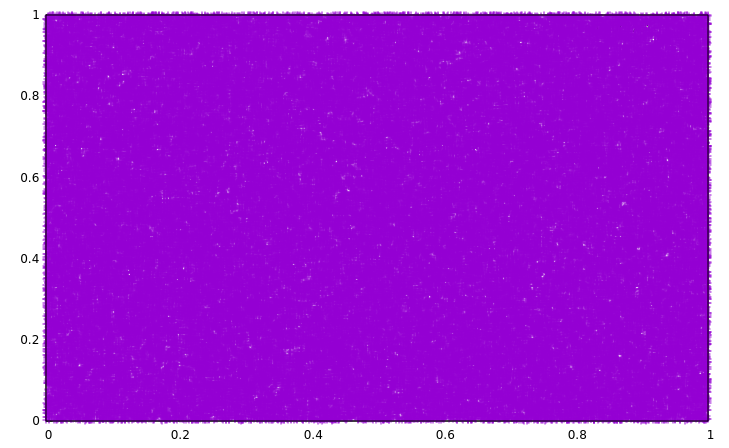
\includegraphics[scale=0.5]{final_plot_full-1}

\item \textbf{Plot of values \(u_i\) from (0,\ 0.001)\ :}\
count=100000\
After zooming it still looks like points are on a certain hyperplane but number of hyperplanes are quite good.

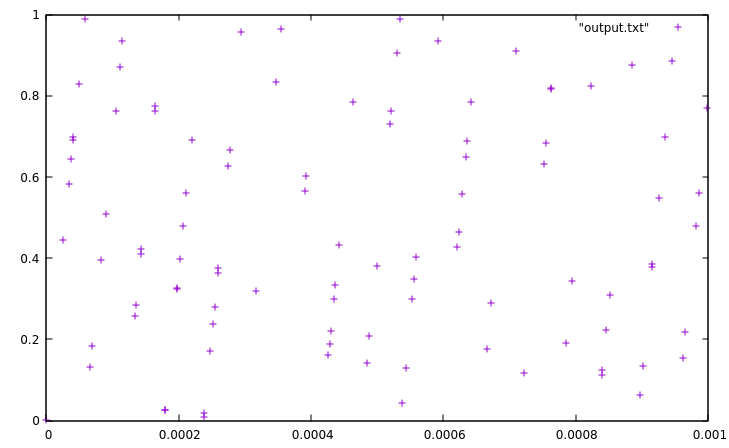
\includegraphics[scale=0.5]{final_plot-1}

\item \textbf{Code: }\


\VerbatimInput{ass3-quest1.cpp}

\end{itemize}
\vspace{5mm}

\section{Question-2}


\[R_k=(\sum_{t=k+1}^{T} (Y_t-\bar{Y})(Y_{l-k}-\bar{Y}))/(\sum_{t=1}^{T} (y_t-\bar{Y})^{2})\]

Since the denominator and numerator contain different number of terms, in particular as the number of terms in the numerator is decreasing in time lag "K". Thus the estimator looks biased and for the large values of k \(R_k\) will vanish.\textbf{But this is what actually wanted.}




\textbf{Plus autocorrelation of Fibonacci generator is more close to zero than that of LCG. Therefore
Fibonacci generator is better than the given LCG in terms of autocorrelation.}

\
\
\
\

Autocorrelation of lag 1, with 1000 generated values, is -0.0355444.\

Autocorrelation of lag 2, with 1000 generated values, is -0.0508289.\

Autocorrelation of lag 3, with 1000 generated values, is -0.0167786.\

Autocorrelation of lag 4, with 1000 generated values, is 0.0189976.\

Autocorrelation of lag 5, with 1000 generated values, is -0.0254554.\

The sample mean for 1000 values is 0.493665.\

The sample variance for 1000 values is 0.0827854.





\textbf{Code: }\

\VerbatimInput{ass3-quest2.cpp}


\end{document}